% partie logiciel:
% 2D

% 3D 1: intersection de demi-espaces -> associer plane + inter pour AD (lien avec AD), type de nombre
% 3D 2: inclusion-exclusion
% -> environ 3 pages + bouts de codes

\chapter{Introduction}

A 3D scanner is a commonly used device that can measure 3D points on the surface
of a physical object.  It produces point clouds that can then be used to create
more complex and complete digitalized models such that meshes. Several methods
exist to build a mesh from a point cloud such that the one described in
\cite{alexa2003computing}. But an important problem may arise when processing
point clouds: since the 3D scanner is a physically-based device, error can be
made during the measurement: the resulting point cloud will be noisy. In this
work, we are interested in removing noise from point clouds: we call this
technique denoising or smoothing.

There is also another issue: we only deal with points and so we can not use all
the techniques developed in image processing like the Fourier transform,
wavelets... A common way of removing the noise from an image is to take its
Fourier transform and filter the high frequencies. For applying the filter, we
need a notion of neighbours and thus some kind of parametrization. An image can
be easily parametrized using a grid of pixels.  When we have a mesh, we have a
kind of parametrization but when we have only points, we do not have such
parametrization.

Several methods already exist to remove noise and get smooth point clouds.
They come from different fields: Computer Vision, Computational Geometry...

\begin{itemize}
    \item \textit{Gaussian / Laplacian smoothing}: each point is replaced by
        another point computed from the nearest neighbours of that point. In
        the Laplacian case, the new point is a convex combination of the
        neighbours (see \cite{vollmer1999improved}).
    \item \textit{Jet fitting} (see \cite{cazals2005estimating}): a jet is a truncated
        Taylor expansion. Such jets are fitted around points. Jet smoothing
        operates by projecting the input points on an estimated smooth
        parametric surface (the so-called jet surface). Jets are good because
        they intrinsically contain differential information such as normal,
        curvature...
    \item \textit{Bilateral smoothing} (see \cite{huang2013edge}): the algorithm
        works by first resampling away from the edges i.e. smooth the point
        cloud around the edges. The second phase of the algorithm consists in
        inserting points by projecting each point onto the implicit surface
        patch fitted over its $ k $ nearest neighbours. This smoothing algorithm
        take into account the sharp edges present in the point set.
\end{itemize}

During this internship, we will use the following idea: suppose we want to
smooth a surface, to do so, one could move each point in the direction of the
normal to the surface by a quantity related to the mean curvature at that point.
The sign of the mean curvature only depends on the choice of the orientation of
the normal.  The more curved the surface is, the more important the displacement
will be. It turns out that the evolution of the surface thus produced can be
modelled with a partial differential equation. If we have a family of surfaces $
S_t $ given by $ x(t, u) $ for $ t \geq 0 $ that satisfies the following
equation:

$$ \partiald{x(t, u)}{t} = \vec{\kappa}(t, u) $$

where $ \vec{\kappa}(t, u) $ is the mean curvature vector of $ S_t $ at $ u $
(see the proposition \ref{prop:curvatures-surface} for a more complete
definition) then we say that the family of surfaces evolves by
mean curvature flow. This family is called the mean curvature flow (MCF) of the
initial surface.

This partial differential equation can be seen as the geometric equivalent of
the heat equation: indeed, the Laplacian is replaced by the mean curvature
vector. Both of them are sums of eigenvalues of some matrices: the Hessian for
the first one and the Shape operator for the second.

The MCF is well-known for its smoothing properties (see
\cite{ciomaga2010level}). For example, the figure
\ref{fig:mean-curvature-flow-ex} is an illustration of the mean curvature flow
on a noisy surface (extracted from \cite{clarenz2000anisotropic}).

\begin{figure}[h]
    \centering
    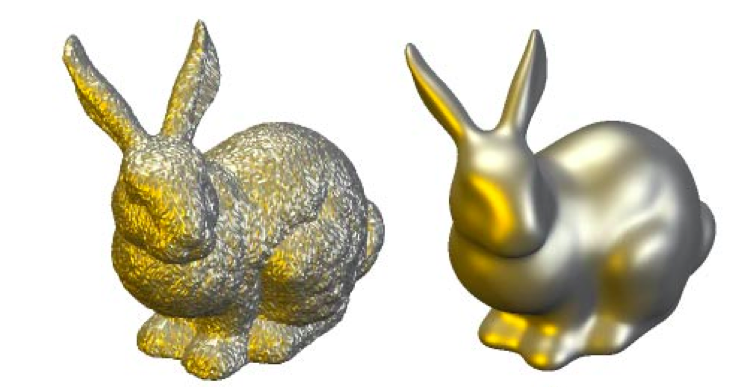
\includegraphics[scale=0.3]{img/mean-curvature-flow-rabbit}
    \caption{Mean curvature flow on a noised surface}
    \label{fig:mean-curvature-flow-ex}
\end{figure}

We will show in the last chapter of this report that this flow is related to the
variation of the area of the surface. If we try to transform the surface while
minimizing the area, we will obtain the same evolution as the one given by the
MCF. But let us keep in mind that we do not know the surface, only a finite set
of points that sample the surface. So, we will need a way to compute the area
without knowing the original surface. A common way of doing so is to consider
the volume of a union of balls centered on the points of the cloud.  We will
show that this quantity is proportional, under some conditions, to the area of
the underlying surface. Thus, it suffices to minimize the volume of this union
of balls to minimize the area of the underlying surface. We will call this
volume the energy $ E(P) $ associated to the point cloud $ P = \{ p_1, \ldots,
p_N \} $.

Now that we have our energy, we need to minimize it. If we are in
three dimensions then we can see the energy $ E $ as a function $ E : \R^{3N}
\to \R $. The main technique used for minimizing a function are based on the
computation of the gradient of the said function. So, we will need a way to
compute the gradient of $ E $. There are many possibilities of doing it:
using exact formulae if they exist, using finite differences...

In this report, we will use an original technique called \textit{Automatic
    Differentiation}. This technique is described in more details in the
appendix \ref{appendix:ad}. In short, it is a technique allowing us to compute
the derivatives of any computer program. It exploits the fact that any program
can be thought of as a sequence of basic arithmetic operations and elementary
functions. Now, using the chain rule and number type overloading we can compute
derivatives of any order without changing too much the cost of the original
function.  This will allow us to only take care of the computation of $ E(P) $
and not of its gradient. This will also allow us to consider different kind of
energies: the volume of the union of balls, the area of the boundary of the
union and also anisotropic ones. Let us detail the latter point.

Anisotropic smoothing is a type of smoothing where the magnitude will depend on
the point and the topology of its neighbourhood. In image processing, this
technique is called anisotropic diffusion (see \cite{weickert1998anisotropic}):
it reduces the image noise without removing significant parts of the image such
as edges, lines...

During this internship, we were interested in a kind of anisotropic evolution
based on \cite{chambolle2012nonlocal} where the smoothing is adapting in
function of the direction: smoothing will be stronger in some privileged
directions. These directions will be given by the user.

Anisotropic flow may have applications that we did not have time to explore
during this internship. It could be used, for example, in physically based
simulations like crystal growth simulation. Another example would be when we
build a 3D scan of an object: we want to be able to smooth the point cloud while
preserving certain details (the signature of the author for example).

This report is structured as follows: first, we will be interested in the two
dimensional case where we will show that our discrete MCF is able to smooth a
point cloud and can be used to estimate the mean curvature vector. Then, we will
look at the 3D case where we will study the anisotropic flow. The final part
will be dedicated to the theory: we will show that the constructed discrete MCF
is effectively an approximation of the continuous MCF.

% vim: set spelllang=en :

